\section{Coût et Redondance}

\begin{frame}
	\frametitle{Coût}
	\begin{block}{Définition}
		Durée d'utilisation d'un canal dans la transmission d'un message.
		\begin{itemize}
			\item Téléphone: Temps de communication.
		\end{itemize}
	\end{block}
	\begin{alertblock}{Economie}
		\centering
		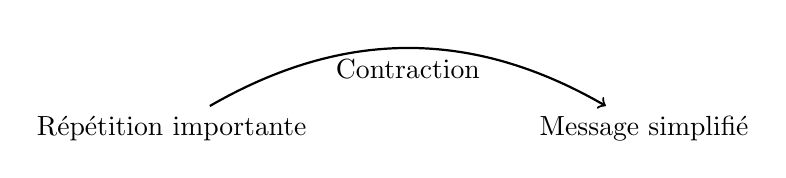
\begin{tikzpicture}
			\node (R) at(0,0) {Répétition importante};
			\node (M) at(6,0) {Message simplifié};
			\draw[->, thick] (R) to[bend left] (M);
			\node at(3,.75) {Contraction};
		\end{tikzpicture}
	\end{alertblock}
	\begin{exampleblock}{Exemples}
		\begin{itemize}
			\item Métro (\emph{Métropolitain}),
			\item Périph (\emph{Boulevard Périphérique}),
			\item Labo (\emph{Laboratoire}),
			\item USA, OGM, Bio...
		\end{itemize}
	\end{exampleblock}
\end{frame}

\begin{frame}
	\frametitle{Coût}
	\begin{alertblock}{Risques}
		\centering
		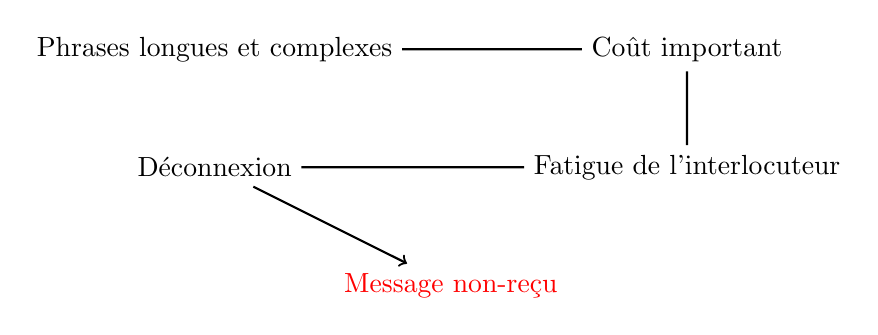
\begin{tikzpicture}
			\node (P) at (0,1.5) {Phrases longues et complexes};
			\node (C) at (6,1.5) {Coût important};
			\node (F) at (6,0) {Fatigue de l'interlocuteur};
			\node (D) at (0,0) {Déconnexion};
			\node[color=red] (R) at (3,-1.5) {Message non-reçu};
			\draw[->, thick] (P)--(C) (C)--(F) (F)--(D) (D)--(R);
		\end{tikzpicture}
	\end{alertblock}
	\begin{exampleblock}{Conséquence}
		\[ \text{Diminuer le nombre de signes} \implies \text{Message plus compréhensible} \]
		$\implies$Exemple: Télégramme.
	\end{exampleblock}
\end{frame}
\begin{frame}
	\frametitle{Efficacité}
	\begin{alertblock}{Problèmes}
		\begin{itemize}
			\item Bruits et parasites (environnement par exemple),
			\item Pertes d'information (discours hâché au téléphone)...
		\end{itemize}
		Equilibre nécessaire entre coût et qualité de réception.
	\end{alertblock}
	\begin{block}{Finalement}
		\begin{itemize}
			\item Ni trop bref,
			\item Ni trop complexe.
		\end{itemize}
	\end{block}
\end{frame}
\begin{frame}
	\frametitle{Efficacité}
	\begin{exampleblock}{Facteurs}
		\begin{columns}
			\begin{column}{.6\textwidth}
				Fréquence d'utilisation des mots:
				\vspace{-0.2cm}
				\begin{columns}
				\small
				\begin{column}{0.45\textwidth}
				\begin{itemize}
					\item Noms: $20\%$,
					\item Verbes: $17\%$,
					\item Adjectifs: $7{,}5\%$,
				\end{itemize}
				\end{column}
				\begin{column}{0.55\textwidth}
				\begin{itemize}
					\item Adverbes: $5{,}5\%$,
					\item Mots "outils": $50\%$.
				\end{itemize}
				\end{column}
				\end{columns}
			\end{column}
			\begin{column}{.4\textwidth}
				\[ \text{Trop de noms} \implies \text{Difficile} \]
			\end{column}
		\end{columns}
	\end{exampleblock}
	\begin{block}{Rendre le discours compréhensible}
		\emph{Degré d'intelligibilité} d'un message:
		\begin{itemize}
			\item Fréquence d'apparition,
			\item Nature des mots.
		\end{itemize}
		Importance de la répartition des informations selon la \emph{fréquence d'apparition} des termes et leur \emph{prévisibilité}.\\
		\bfseries \textcolor{red}{2 Exemples en opposition.}
	\end{block}
\end{frame}
\begin{frame}
	\frametitle{Redondance}
	\begin{block}{Objectifs}
		\begin{itemize}
			\item Assurer la qualité de la réception,
			\item Augmenter l'impact sur le récepteur,
			\item Outil de contrôle pour le récepteur.
		\end{itemize}
	\end{block}
	\begin{exampleblock}{Définition}
		Excédent de signes pour une quantité d'information égale.
	\end{exampleblock}
	\begin{block}{Caractéristiques}
		Nécessité:
		\begin{itemize}
			\item Faible dans la communication automatique (entre machines),
			\item Indispensable dans la communication entre humains.
		\end{itemize}

		Conséquence: le \emph{coût}.
	\end{block}
\end{frame}
\begin{frame}
	\frametitle{Redondance}
	\begin{block}{Nécessité}
		Doute:
		\begin{itemize}
			\item Qualité de la réception,
			\item Système de référence,
			\item Code,
			\item Habitudes du récepteur.
		\end{itemize}

		Conditionne l'efficacité.
	\end{block}
	\begin{exampleblock}{Redondance naturelle}
		\begin{itemize}
			\item Geste,
			\item Communication entre personnes.
		\end{itemize}
	\end{exampleblock}
\end{frame}
